\section{Merkmale von Cloud-nativen Anwendungen}
\label{sec:cloud-native-anwendungen}
Mit Cloud-nativen Anwendungen kann das maximale Potenzial des Cloud Computing ausgenutzt werden \cite[Vgl.][]{VMwareb}. So können Produktivität und Effizienz gesteigert, sowie die Anwendungen schneller ausgeliefert werden \cite[Vgl][S. 12]{Chandrasekaran2022}. Im Folgenden werden die Merkmale von Cloud-nativen Anwendungen genauer untersucht.

% Was ist eine Cloud Native Anwendung?
% Merkmale
\subsection{Skalierbarkeit}
Von Cloud-nativen Anwendungen wird unter anderem erwartet, dass diese schnell skalieren können, um einer steigenden Nutzerzahl gerecht zu werden \cite[Vgl.][S. 1ff]{Armbrust2009}\cite[Vgl.][S. 234]{Villamizar2017}. Auf der anderen Seite sollen so die Vorteile der Cloud auch hinsichtlich der Kosten realisiert werden, indem die Services genauso herunter skaliert werden können \cite[Vgl.][S. 884]{Adzic2017}.

Skalierbarkeit bedeutet in diesem Zusammenhang, dass die bereitgestellten IT-Ressourcen, wie Rechen- oder Speicherkapazität an die aktuelle Last angepasst und entsprechen erhöht oder oder reduziert werden können \cite[Vgl.][S. 15]{Reinheimer2018}\cite[Vgl.][]{Geißler2019}. Dabei wird in zwei Arten der Skalierung eines Systems unterschieden: \textbf{vertikale Skalierung} und \textbf{horizontale Skalierung} \cite[Vgl.][]{Geißler2019}\cite[Vgl.][]{VMware}

\begin{figure}[H]
    \centering
    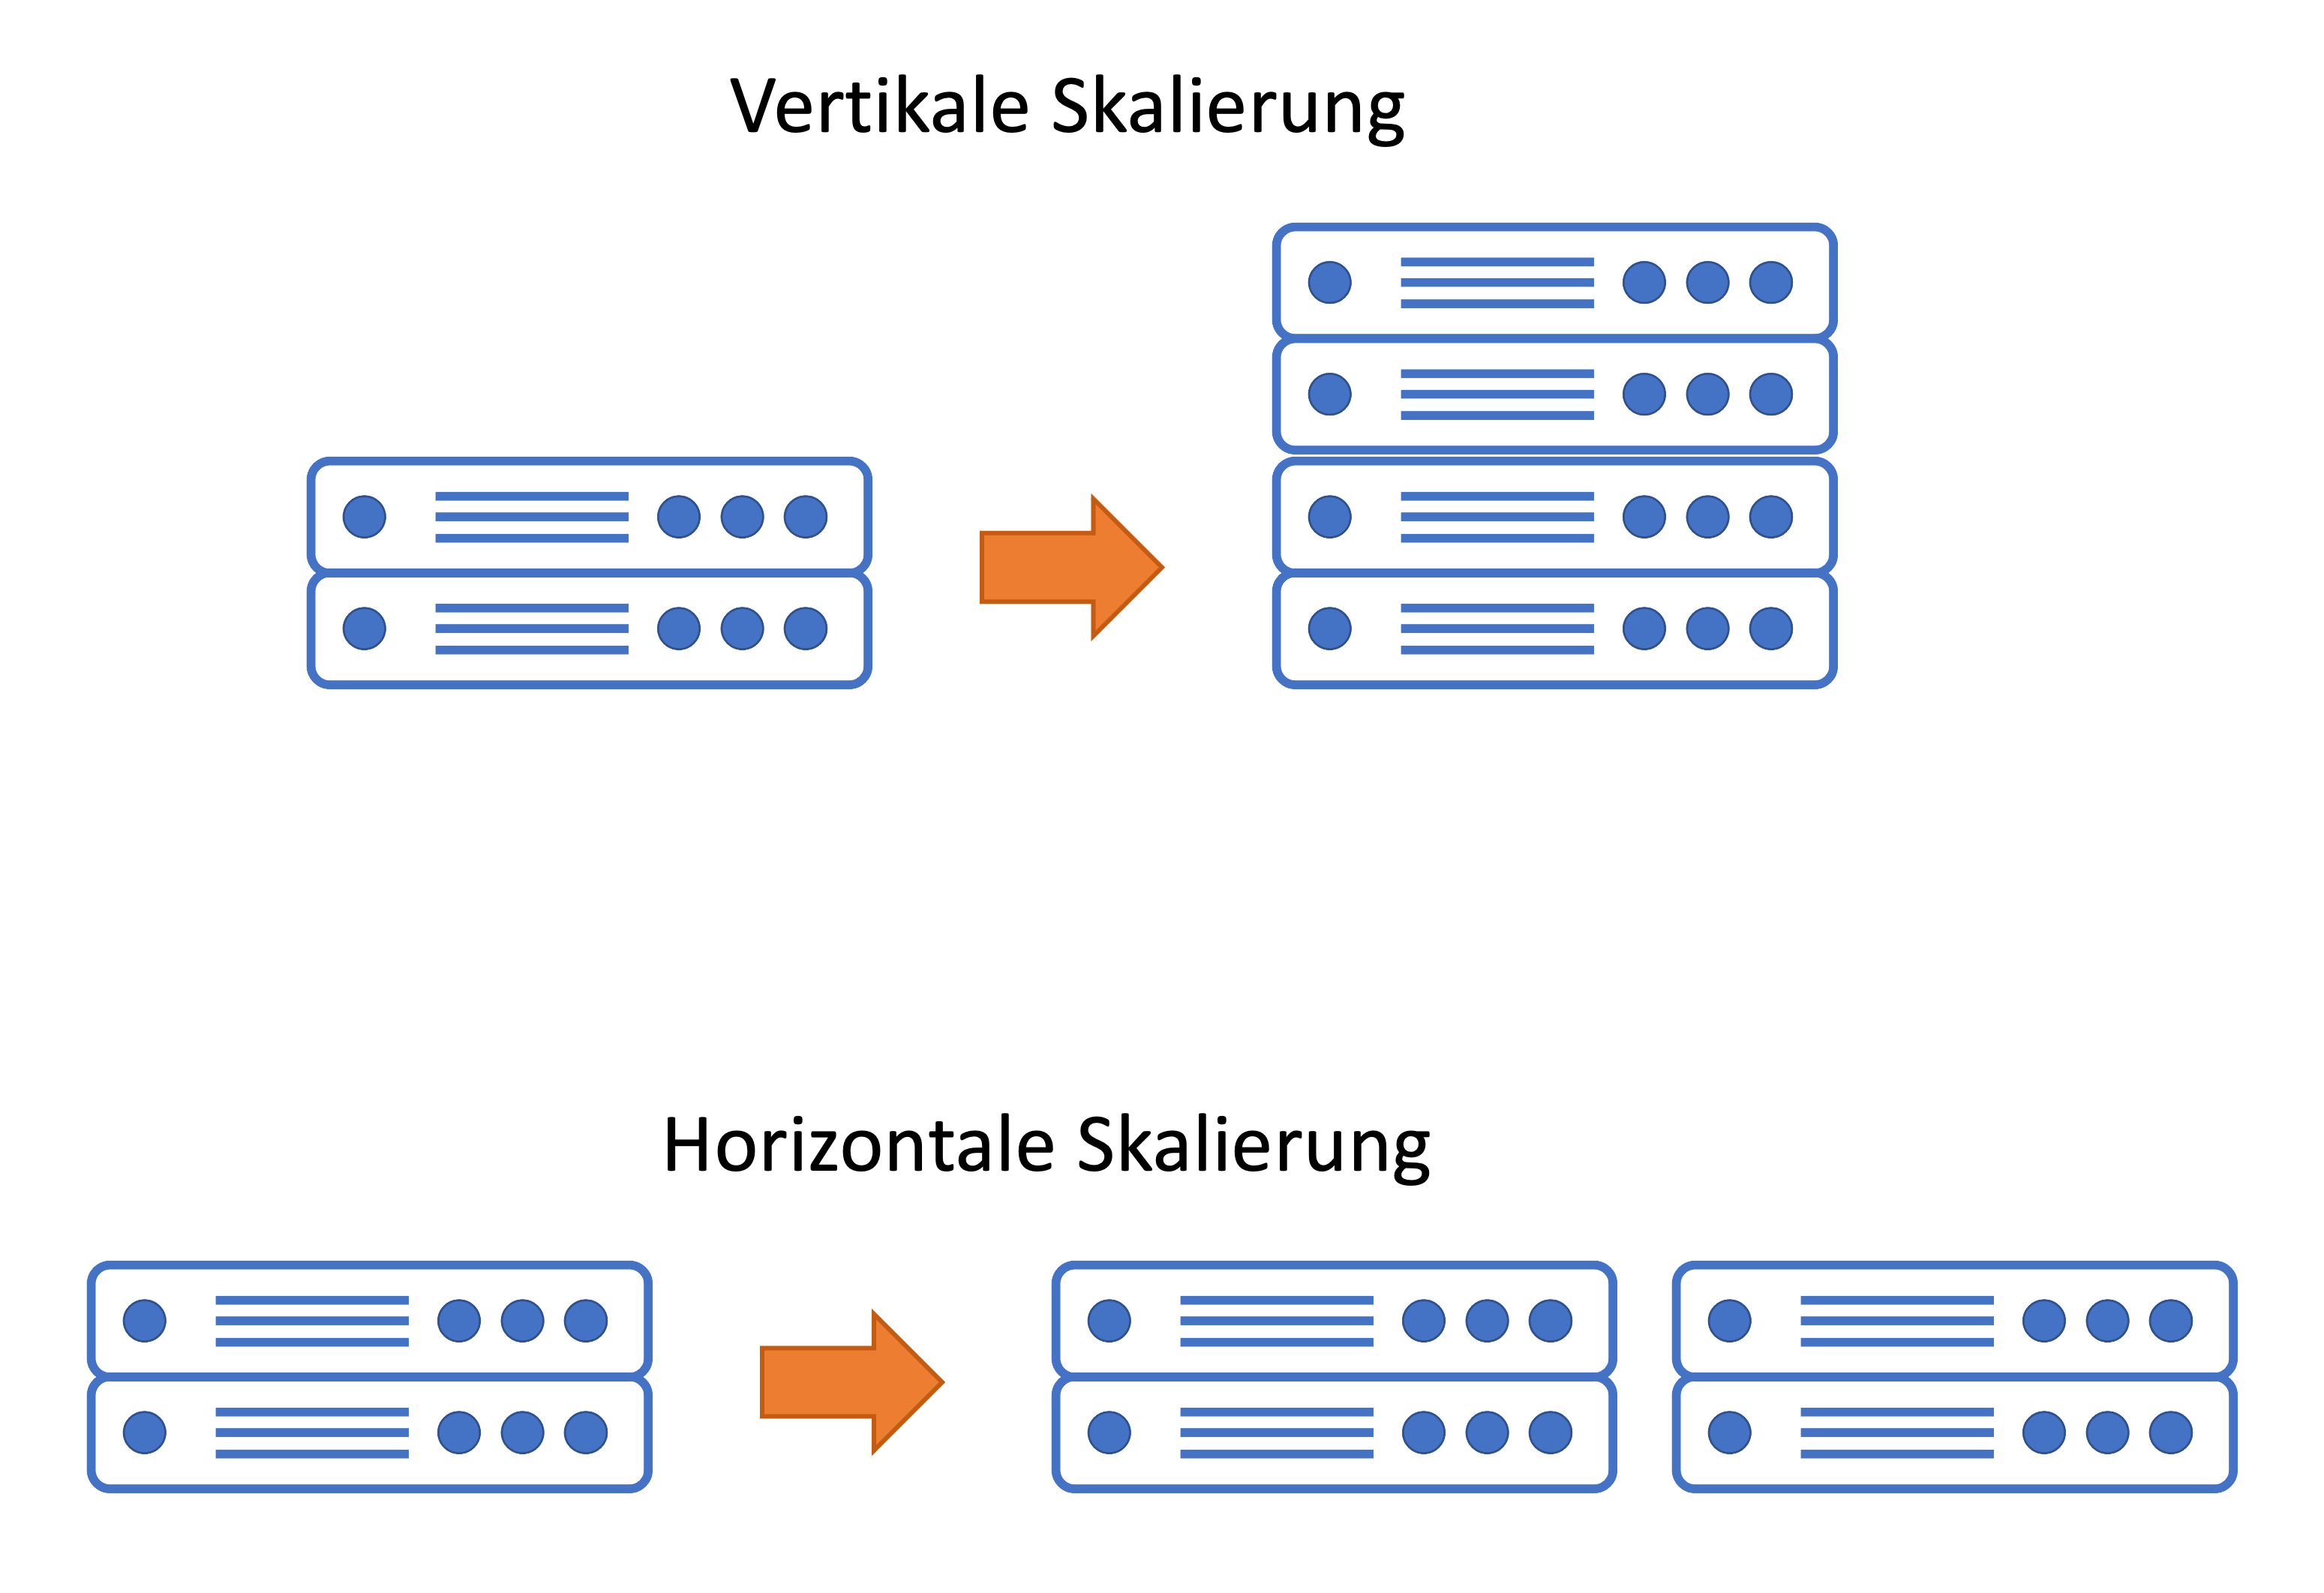
\includegraphics[width=0.65\textwidth]{scale-up_scale-out.png}
    \caption{Vertikale vs. Horizontale Skalierung \cite[Nachbildung nach][]{Bachmann2019}}
    \label{fig:scale-up-scale-out}
\end{figure}
\pagebreak

\textbf{Vertikale Skalierung:}

Bei der vertikalen Skalierung wird zu einer Einheit innerhalb eines Systems zusätzliche Rechenleistung oder zusätzlicher Speicher hinzugefügt. Diese Art der Skalierung wird auch als ''Scale-up'' bezeichnet, abgeleitet von dem Erhöhen der Leistung. Die vertikale Skalierung ist jedoch dadurch limitiert, dass bei der Leistungsaufstockung hardwareseitig Grenzen gesetzt sind \cite[Vgl.][]{Geißler2019}\cite[Vgl.][]{VMware}.

\textbf{Horizontale Skalierung:}

Zur horizontalen Skalierung werden dagegen nicht die Ressourcen innerhalb einer Einheit erhöht, sondern weitere Einheiten beziehungsweise Knoten zu einem System hinzugefügt. Die Aufgaben werden dann auf mehreren Systemen durchgeführt, oder zum Beispiel eine Anwendung in mehreren Containern parallel ausgeführt. Horizontale Skalierung wird auch als ''Scale-out'' bezeichnet, da ein System hier in seiner Breite erweitert wird. In der Theorie sind der horizontalen Skalierung (hardwareseitig) keine Grenzen gesetzt \cite[Vgl.][]{Geißler2019}\cite[Vgl.][]{VMware}.

\subsection{Fehlertoleranz}
Eine weitere Anforderung an Cloud-native Anwendungen ist die Fehlertoleranz. Es sollte grundsätzlich davon ausgegangen werden, dass Fehler auftreten können und diese abgefangen werden müssen \cite[Vgl.][S. 17]{Gannon2017}. Zu diesen Fehlern gehört unter anderem das Abstürzen von Containern und Hardware- oder Netzwerkfehler.
% Auch durch horizontale Skalierung, weil einzelne Nodes ausfallen können

\subsection{Schnelle Bereitstellung}
Mit \textit{Continous Delivery}, zu deutsch kontinuierliche Bereitstellung, können Änderungen in der Anwendung unmittelbar ausgeliefert werden, ohne zum Beispiel auf ein Wartungsfenster nachts warten zu müssen oder die Änderungen mit weiteren Updates zu einem Release zu bündeln, bevor diese ausgeliefert werden \cite[Vgl.][]{VMwareb}. \pagebreak

\subsection{Containerisierung}
Gegenüber der Verwendung von \acp{VM} bieten Container eine höhere Effizienz und Geschwindigkeit. Das Starten und Beenden von Containern ist einer \ac{VM} zeitlich voraus. \cite[Vgl.][]{VMwareb}
% Darüber hinaus benötigt eine \ac{VM} weitere Pakete, da diese die Hardware virtualisiert, wogegen in Containern nur das Betriebssystem virtualisiert wird \cite[Vgl.][]{VMwareb}.
Während \acp{VM} über einen Hypervisor ausgeführt werden, welcher es ermöglicht Hardware auf einem physischen Server zu emulieren und jede \ac{VM} ihre eigenen \textit{Binaries}\footnote{dt. Binärdateien, Dateien, die z. B. kompilierten Code in Maschinensprache enthalten} und \textit{Libraries}\footnote{dt. Bibliotheken, Sammlung von Ressourcen für ein Computerprogramm} besitzt, werden Container auf einem geteilten \textit{Kernel} ausgeführt und können sich diese \textit{Binaries} und \textit{Libraries} somit teilen \cite[Vgl.][]{Jones2018}.

\subsection{Weitere Merkmale}
% Vorhersehbarkeit, kollaborative Entwicklung, Microservices
Weitere Merkmale Cloud-nativer Anwendungen sind unter anderem eine bessere Verlässlichkeit, durch eine gewährleistete ''Ausfallsicherheit'', durch zum Beispiel der Verwendung vieler unabhängiger Microservices (siehe Kapitel \ref{sec:architekturstile}), wodurch auch die Entwicklung in Teams erleichtert wird, da die Services unabhängig voneinander aktualisiert werden können \cite[Vgl.][]{VMwareb}.

Darüber hinaus hat sich auch \textit{Serverless Computing} als Weiterführung des Cloud-native Gedanken etabliert \cite[Vgl.][S. 1]{CNCF2018}, weshalb im anschließenden Kapitel genauer darauf eingegangen wird. \pagebreak